\documentclass{standalone}
%\usepackage[nofragment]{lyluatex}
\usepackage{tikz}
\usepackage{fontspec}

\newcommand{\scoretrack}{
{%
\parindent 0pt
\noindent
\ifx\preLilyPondExample \undefined
\else
  \expandafter\preLilyPondExample
\fi
\def\lilypondbook{}%
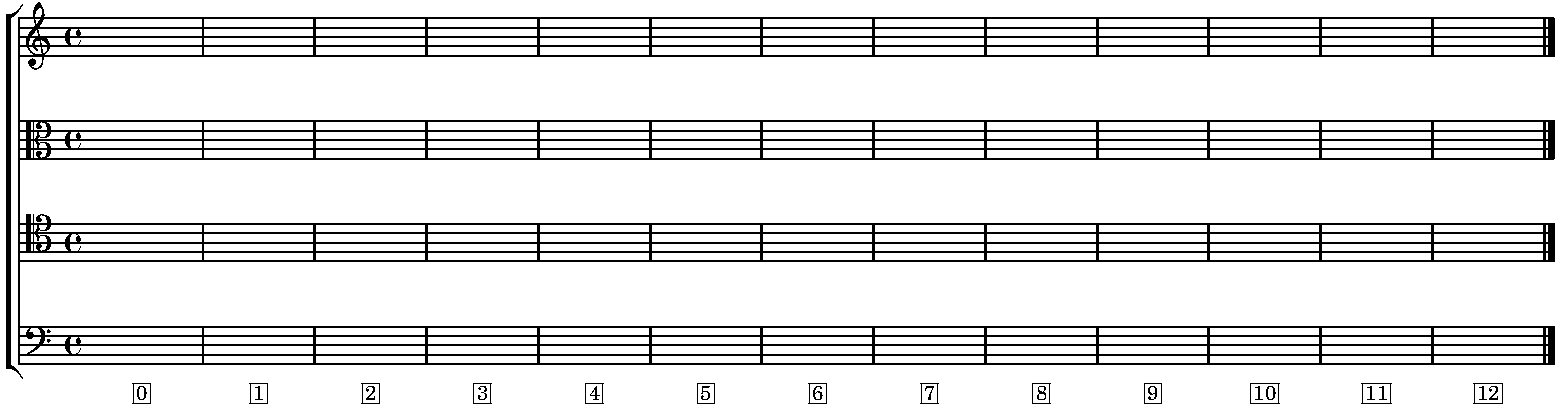
\includegraphics{/Users/mike/Sandbox/GitHubRepositories/TestPiece/1c/lily-865b6703-1}%
% eof
%
\ifx\postLilyPondExample \undefined
\else
  \expandafter\postLilyPondExample
\fi
}
}

\usepackage{graphics}
\begin{document}
\begin{tikzpicture}
\path[draw] (-148.5mm, 0mm) rectangle (148.5mm, -210mm);
\path[draw] (-148.5mm, 0mm) rectangle (148.5mm, -105mm);
\node[anchor=north] at (0, -1.0cm) {{
\setmainfont{Tex Gyre Schola}
\Huge
Test Piece -- Score
}};
\node[anchor=south] at (0, -94mm) {\scoretrack};

\node[anchor=north] at (0, -115mm) {{
\setmainfont{Tex Gyre Schola}
\Huge
Test Piece -- Score
}};
\node[anchor=south] at (0, -199mm) {\scoretrack};

\end{tikzpicture}
\end{document}